%%% Laboratory	 Notes
%%% Template by Mikhail Klassen, April 2013
%%% Contributions from Sarah Mount, May 2014
\documentclass[a4paper]{tufte-handout}

\newcommand{\workingDate}{\textsc{Feb $|$ 2023}}
\newcommand{\userName}{\AE ther Zhou}
% \newcommand{\institution}{Your University}

\usepackage{lab_notes}
\usepackage{siunitx}

\usepackage{hyperref}
\hypersetup{
    pdffitwindow=false,            % window fit to page
    pdfstartview={Fit},            % fits width of page to window
    pdftitle={Lab notes 2014},     % document title
    pdfauthor={Your Name},         % author name
    pdfsubject={},                 % document topic(s)
    pdfnewwindow=true,             % links in new window
    colorlinks=true,               % coloured links, not boxed
    linkcolor=DarkScarletRed,      % colour of internal links
    citecolor=DarkChameleon,       % colour of links to bibliography
    filecolor=DarkPlum,            % colour of file links
    urlcolor=DarkSkyBlue           % colour of external links
}


\title{PHYS 128AL Lab Notebook}
\author[]{\AE ther Zhou}
\date{Feb. 2023}

\begin{document}
\maketitle
%%%%%%%%%%%%%%%%%%%%%%%%%%%%%%%%%%%%%%%%%%%%%%%%%%%%%%%%

\begin{projects}
	\begin{description}
        \item [Lab 2] Cavendish 
		\item [Collaborator] Eric Yang, Kien Le
		\end{description}
\end{projects}

%%%%%%%%%%%%%%%%%%%%%%%%%%%%%%%%%%%%%%%%%%%%%%%%%%%%%%%%
\tableofcontents

\newpage

%%%%%%%%%%%%%%%%%%%%%%%%%%%%%%%%%%%%%%%%%%%%%%%%%%%%%%%%
\section{Daily}
\newday{6 Feb 2023, M}
\begin{itemize}
    \item {equipment set up: } {screen, laser, pendulum}
    \item Method 1
    \item {laser doesn't move} {balance might been stuck by the buffer(provide damping)}
    \item {optic table is not stable enough}
    \item {screen is too close to the device} {(ideally $5\, \si{.m}$ but we only have about $2.4\, \si{.m}$)}
\end{itemize}
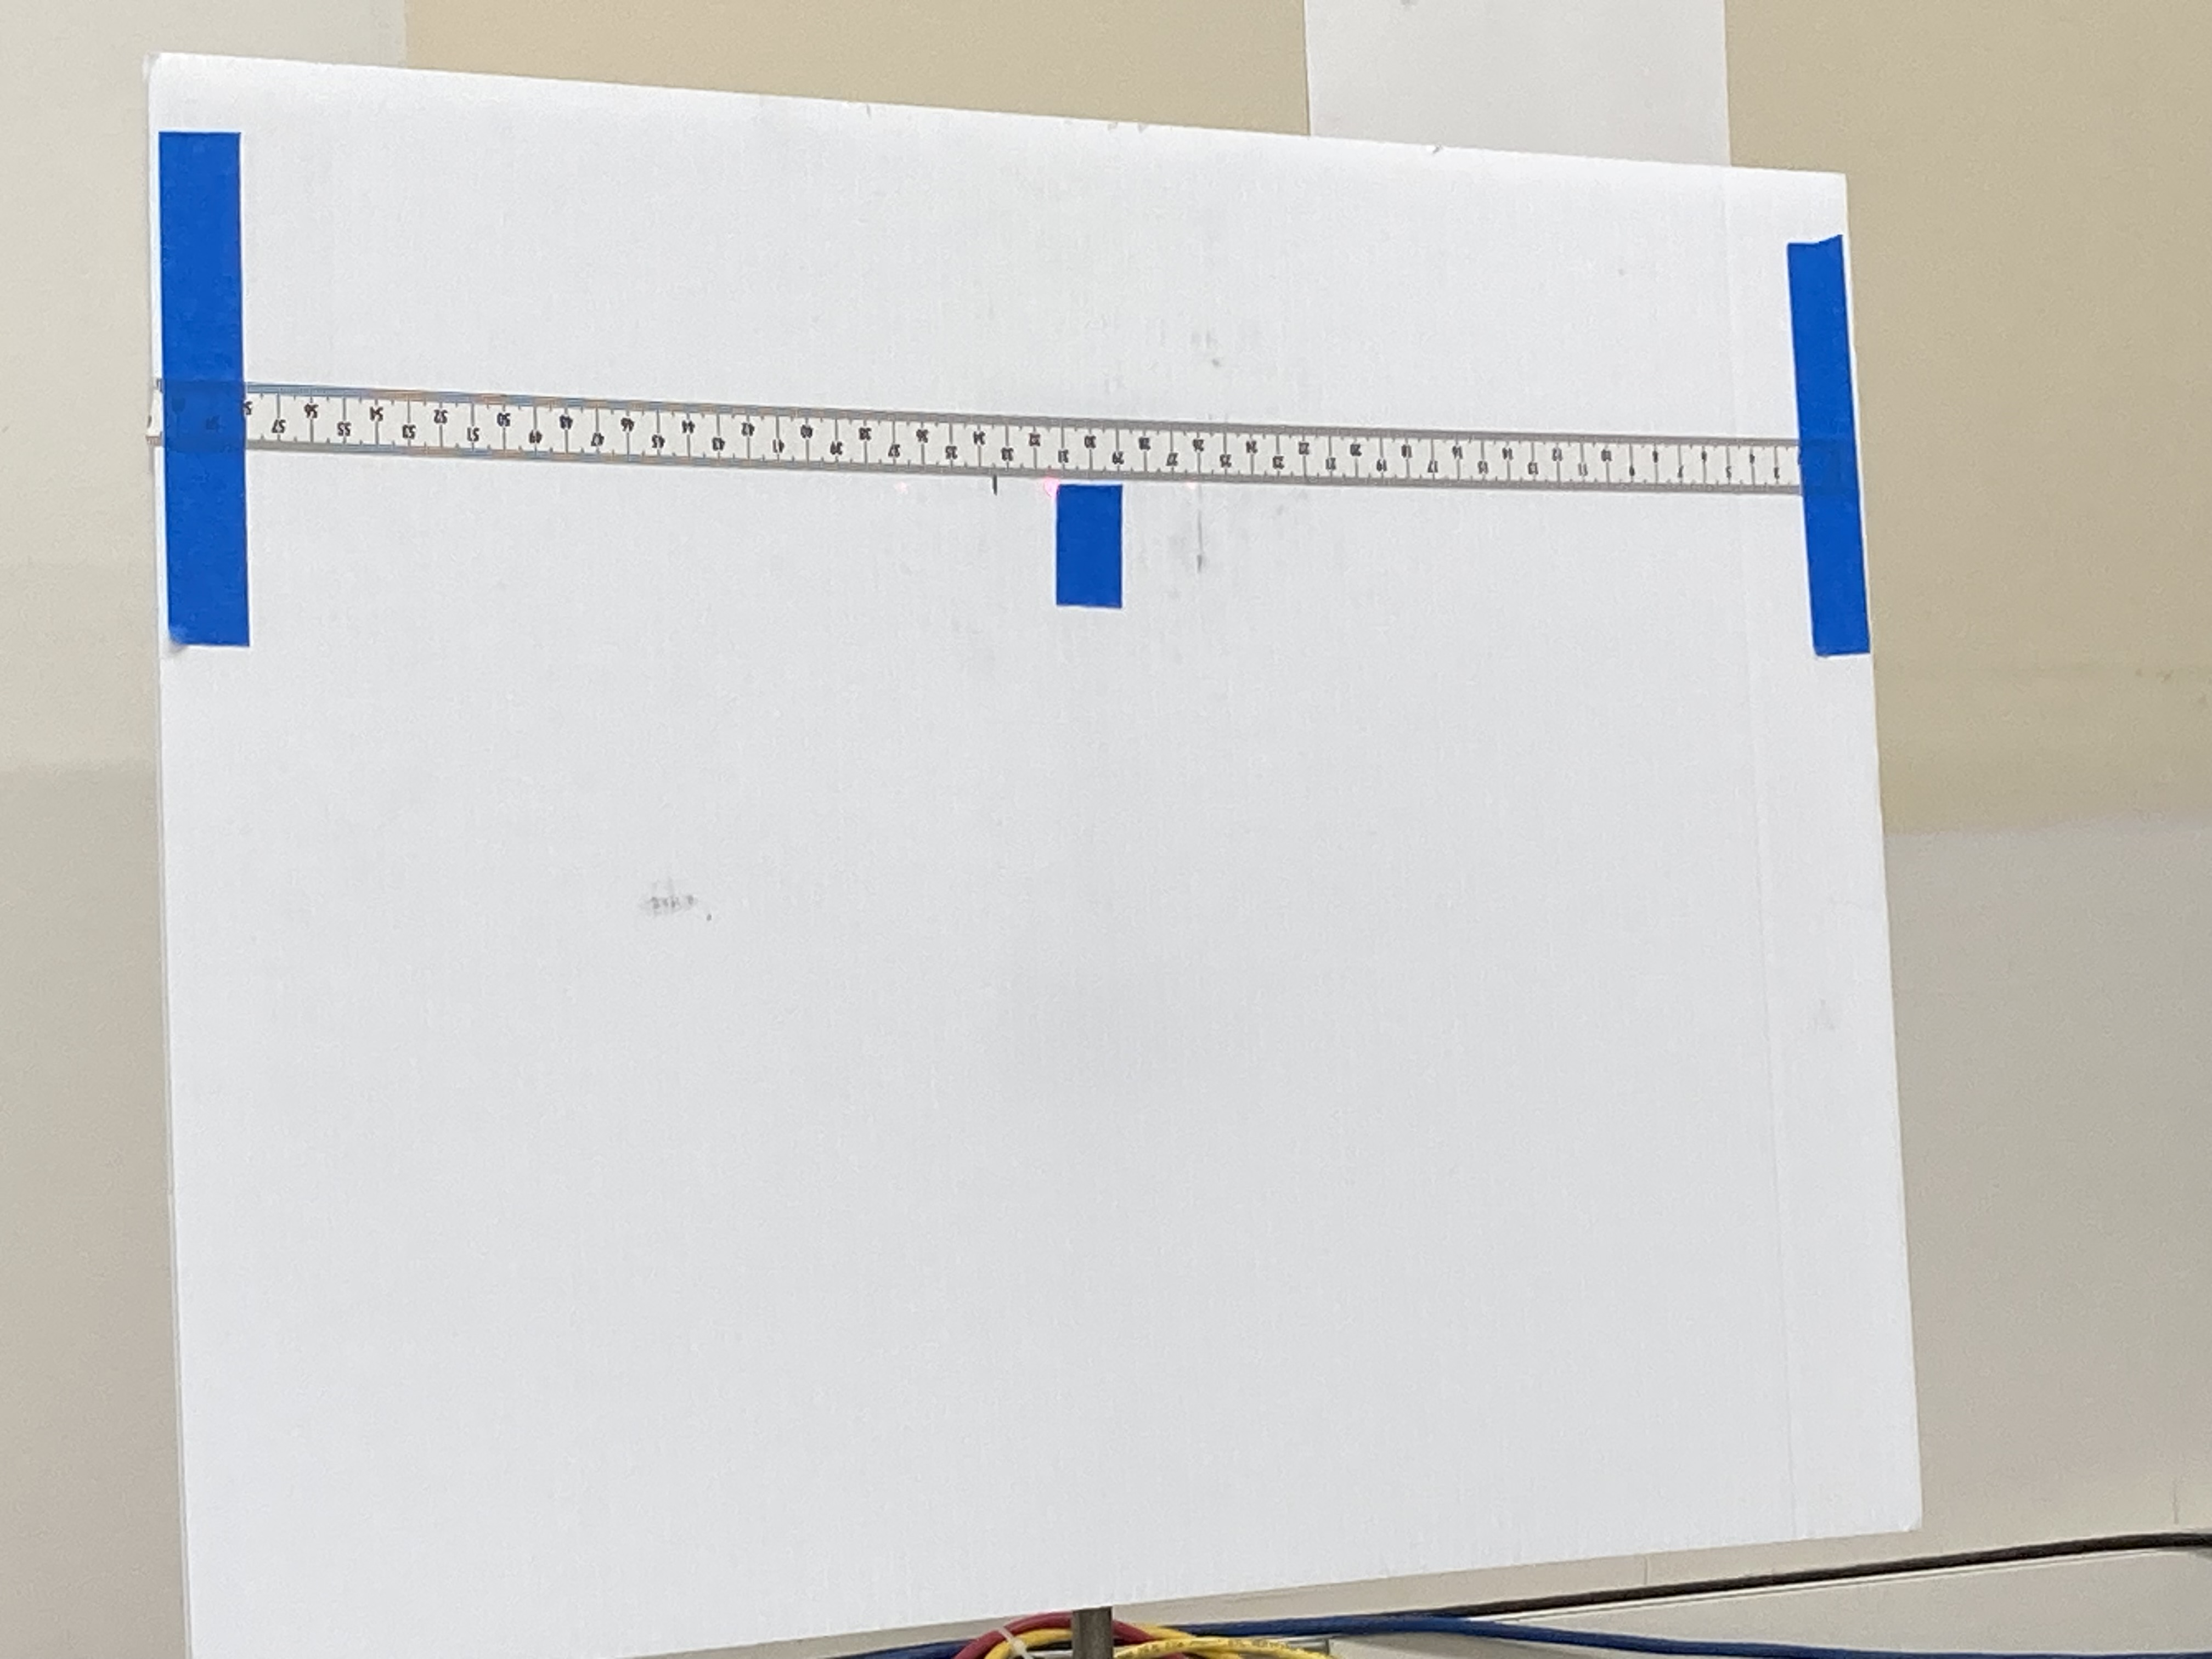
\includegraphics[width = 0.5 \textwidth]{figures/day_1_screen.JPG}
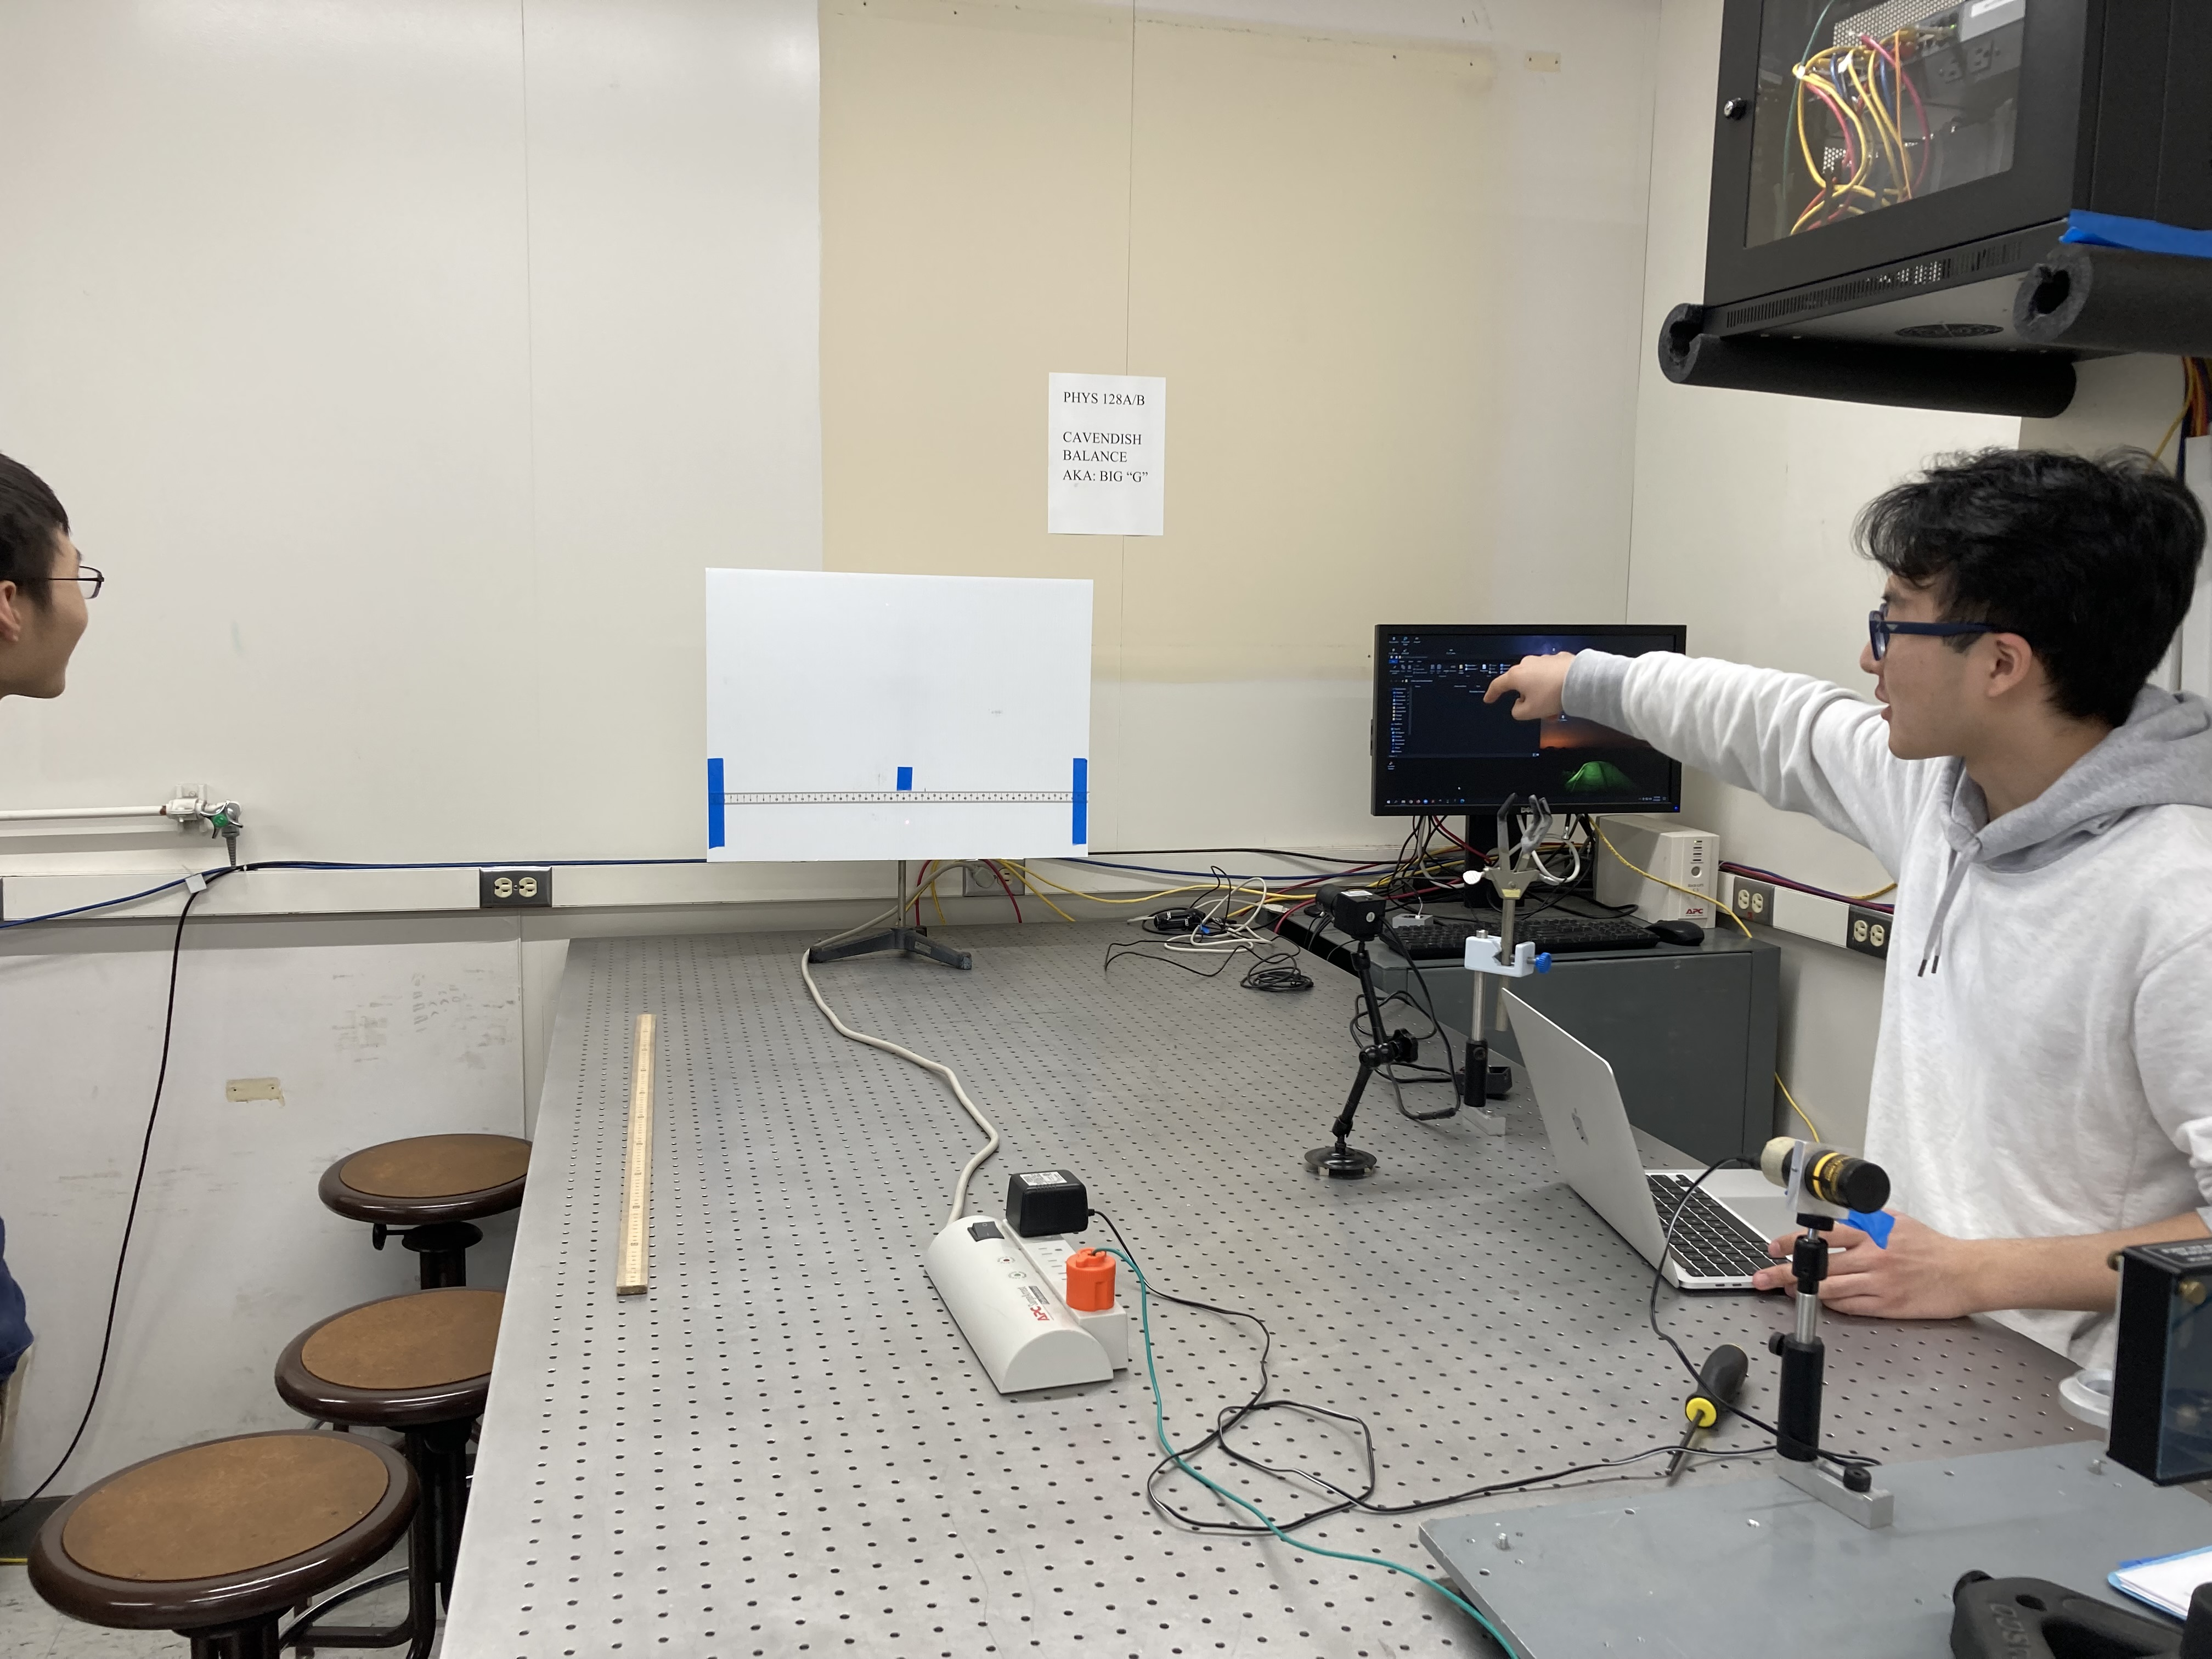
\includegraphics[width = 0.5 \textwidth]{figures/day_1.JPG}

\hrulefill

%%%%%%%%%%%%%%%%%%%%%%%%%%%%%%%%%%%%%%%%%%%%%%%%%%%%%%%%

\newday{8 Feb 2023, W}
Doing Method 3
\begin{itemize}
    \item {equipment set up: } {adjust laser, set up large balls, release pendulum}
    \item {Stabilizing about $S_1$}
    \item {elastic distortion dominate?}
\end{itemize}
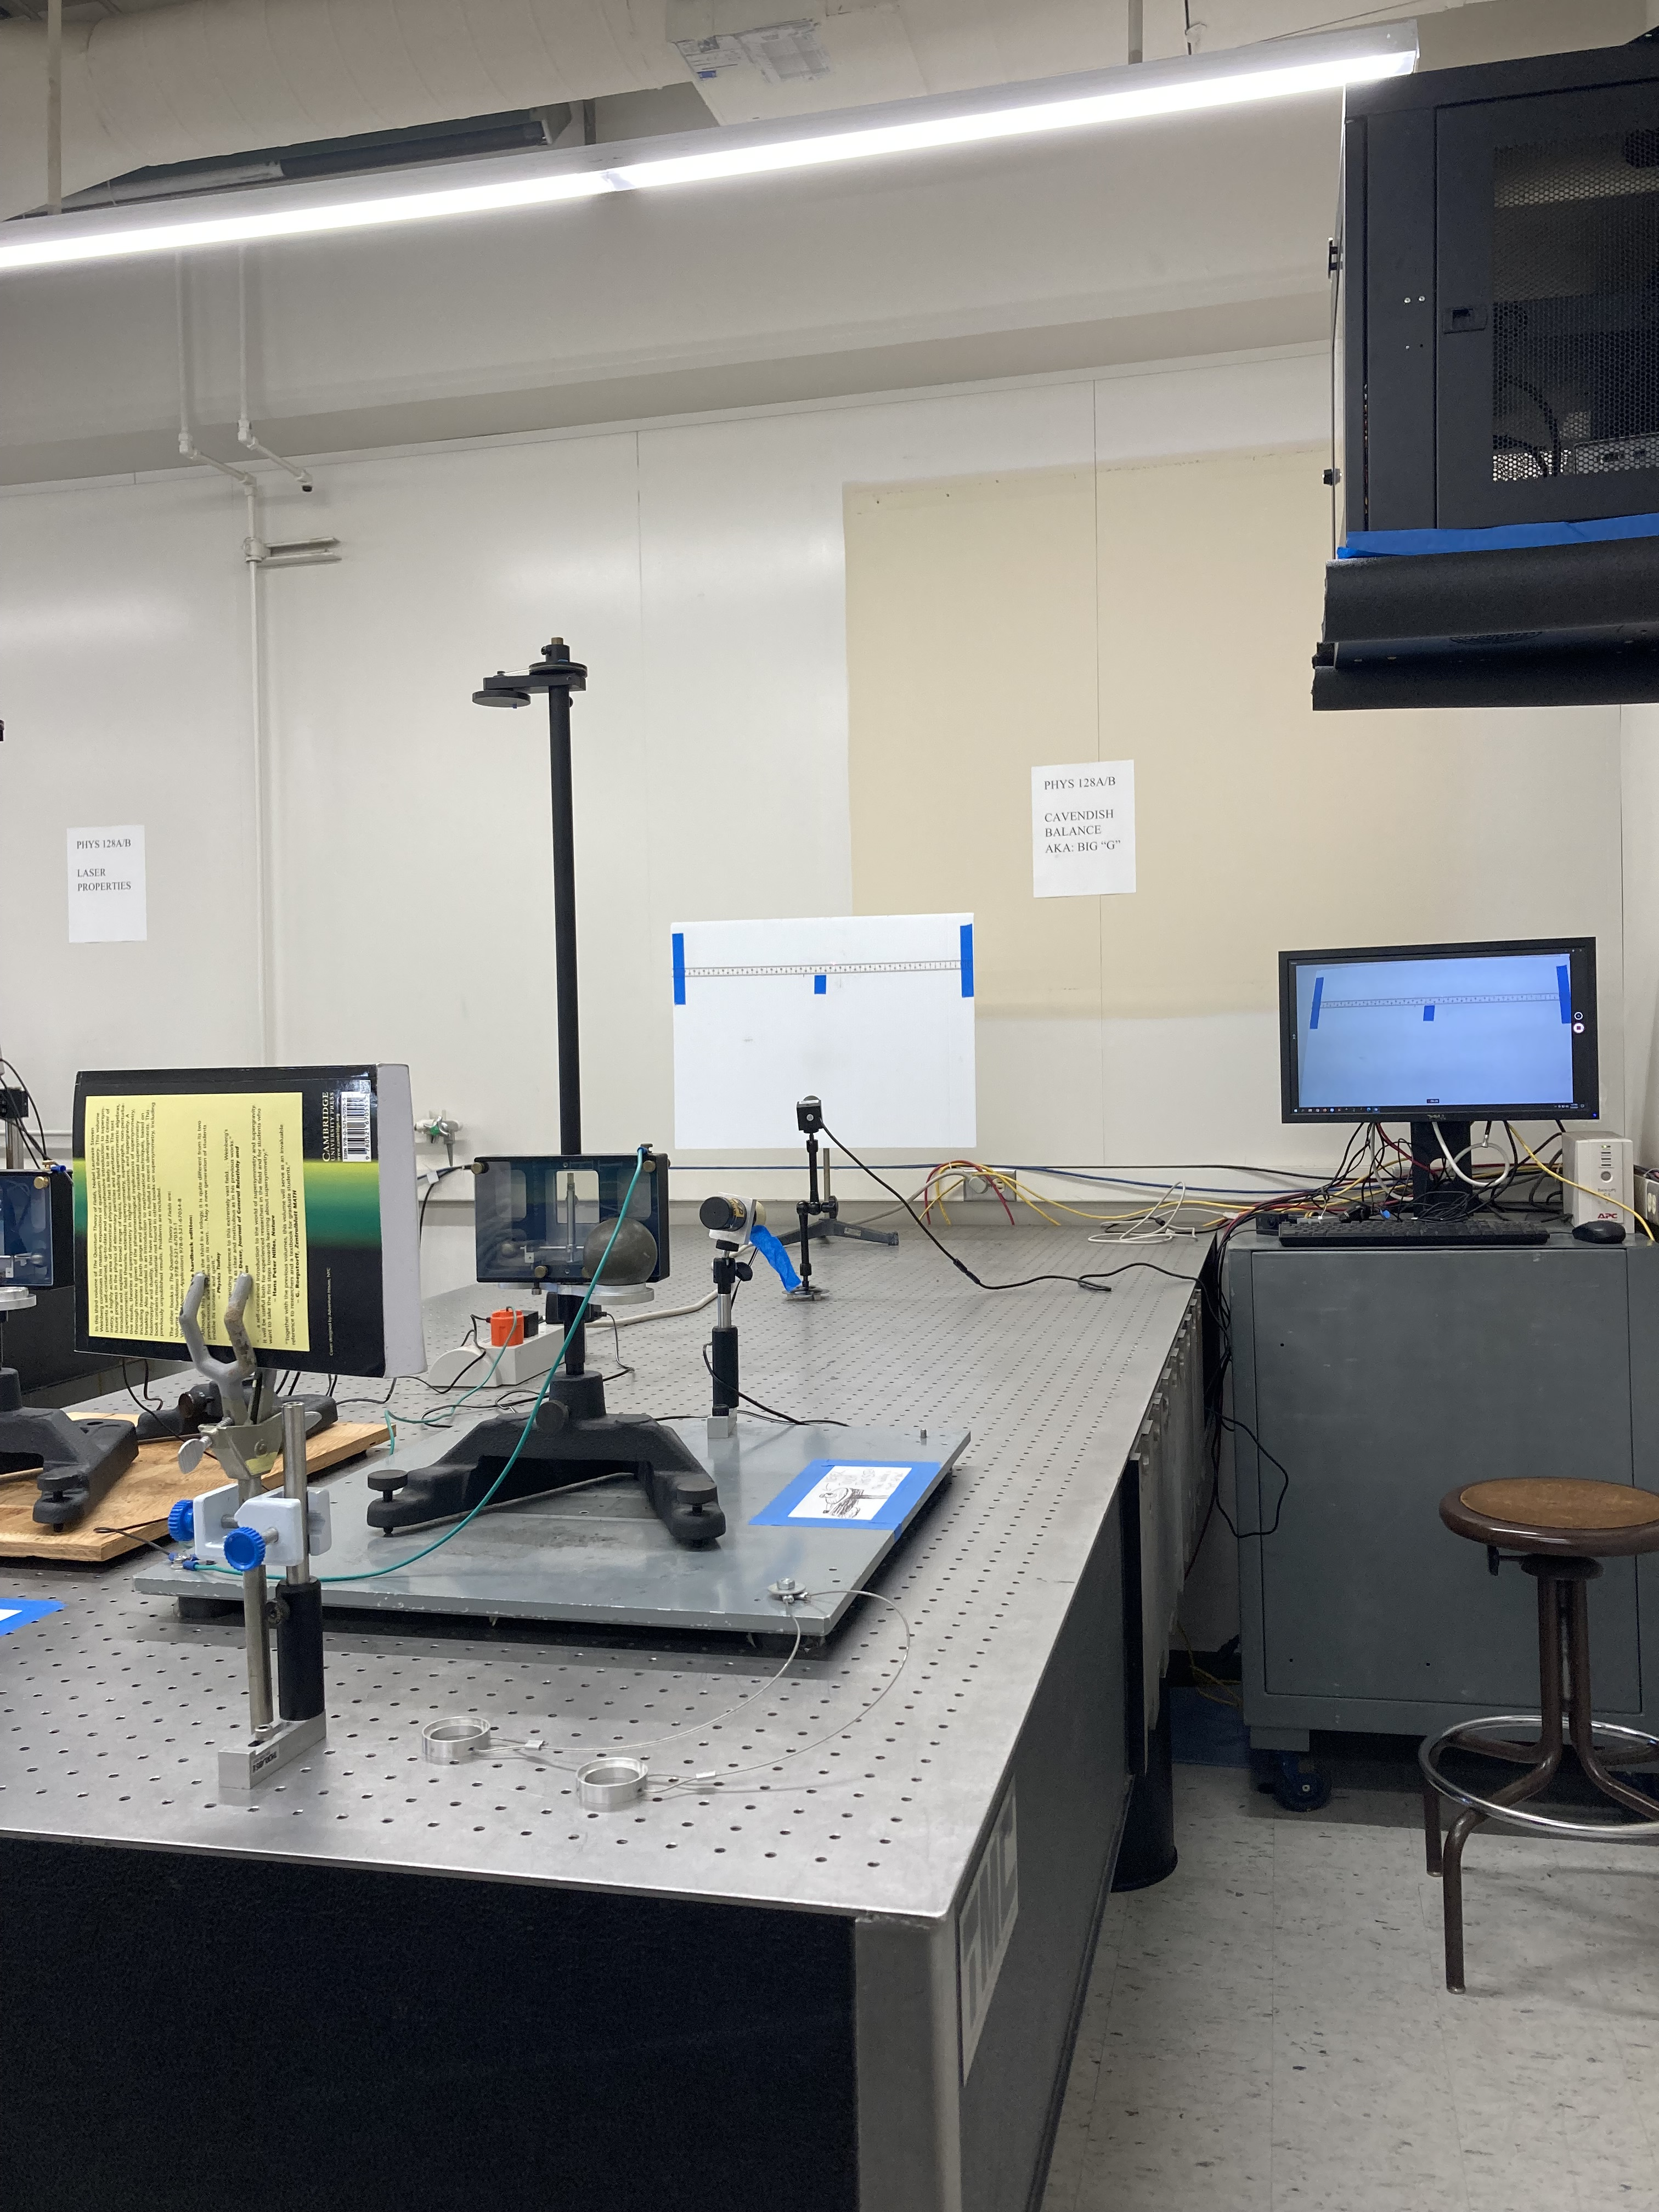
\includegraphics[width = 0.5     \textwidth]{figures/day_2.JPG}

$$\ddot{\theta} = a_{\si{twist}}+g_{\si{mass}}$$
$$a_{\si{twist}} = -k_{\si{elastic}}\cdot \theta$$
$$g_{\si{mass}} = G\cdot m_1\cdot \theta^{-2}$$\
Let $G_m = G\cdot m_1$
$$\ddot{\theta} = -k_e\cdot \theta+G_m\cdot \theta^{-2}$$
For perturbation $\delta \theta$ near equilibrium position $\ddot{\theta} = 0$
$$\delta \ddot{\theta} = -k_e\cdot \delta \theta + G_m \cdot \left(-2\delta \theta/ \theta^3+ \cdots \right)$$

Here we post a few column of our raw data

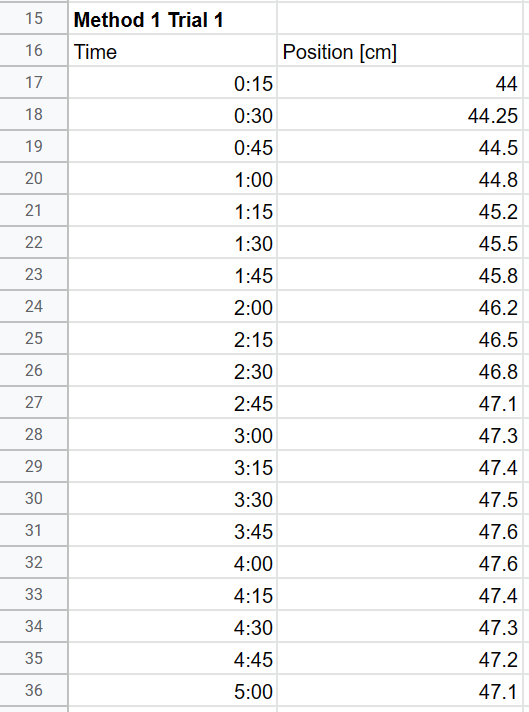
\includegraphics[scale=0.65]{figures/raw_feb8.png}

with systematic error in time and position. For time measuring, error is about 1 second. For position measuring, error is about $0.1$ centimeter.

\hrulefill

%%%%%%%%%%%%%%%%%%%%%%%%%%%%%%%%%%%%%%%%%%%%%%%%%%%%%%%%
\newday{13 Feb 2023, M}
read data from video

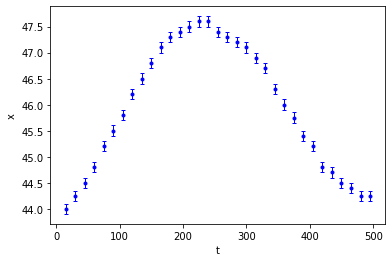
\includegraphics[scale=0.65]{figures/data_feb8.png}

With \Python{scipy.curve\_fit()} Fitted data to get acceleration

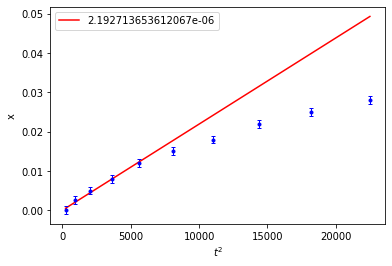
\includegraphics[scale=0.65]{figures/fit_feb8.png}

By method 3, we calculated gravitational constant
$$G=3.04\times 10^{-11} \,\si{.m^2\cdot kg^{-1}\cdot s^{-2}}\approx \frac{1}{2}G_{\si{N}}$$

\hrulefill

%%%%%%%%%%%%%%%%%%%%%%%%%%%%%%%%%%%%%%%%%%%%%%%%%%%%%%%%
\newday{15 Feb 2023, W}
We calibrated the equipment for several hours and recorded the oscillation around equilibrium positions. After that, we read data from the video records manually, and measured equilibrium positions ($S_1$ and $S_2$). 

These row data are subjected to error in position ($\pm 0.2\, \si{cm}$) and in time ($\pm 1.0 \, \si{sec}$). Error in position is given by radius of the laser dot on our screen of measurement, and the error in time is given by minimum time scale of our video records.

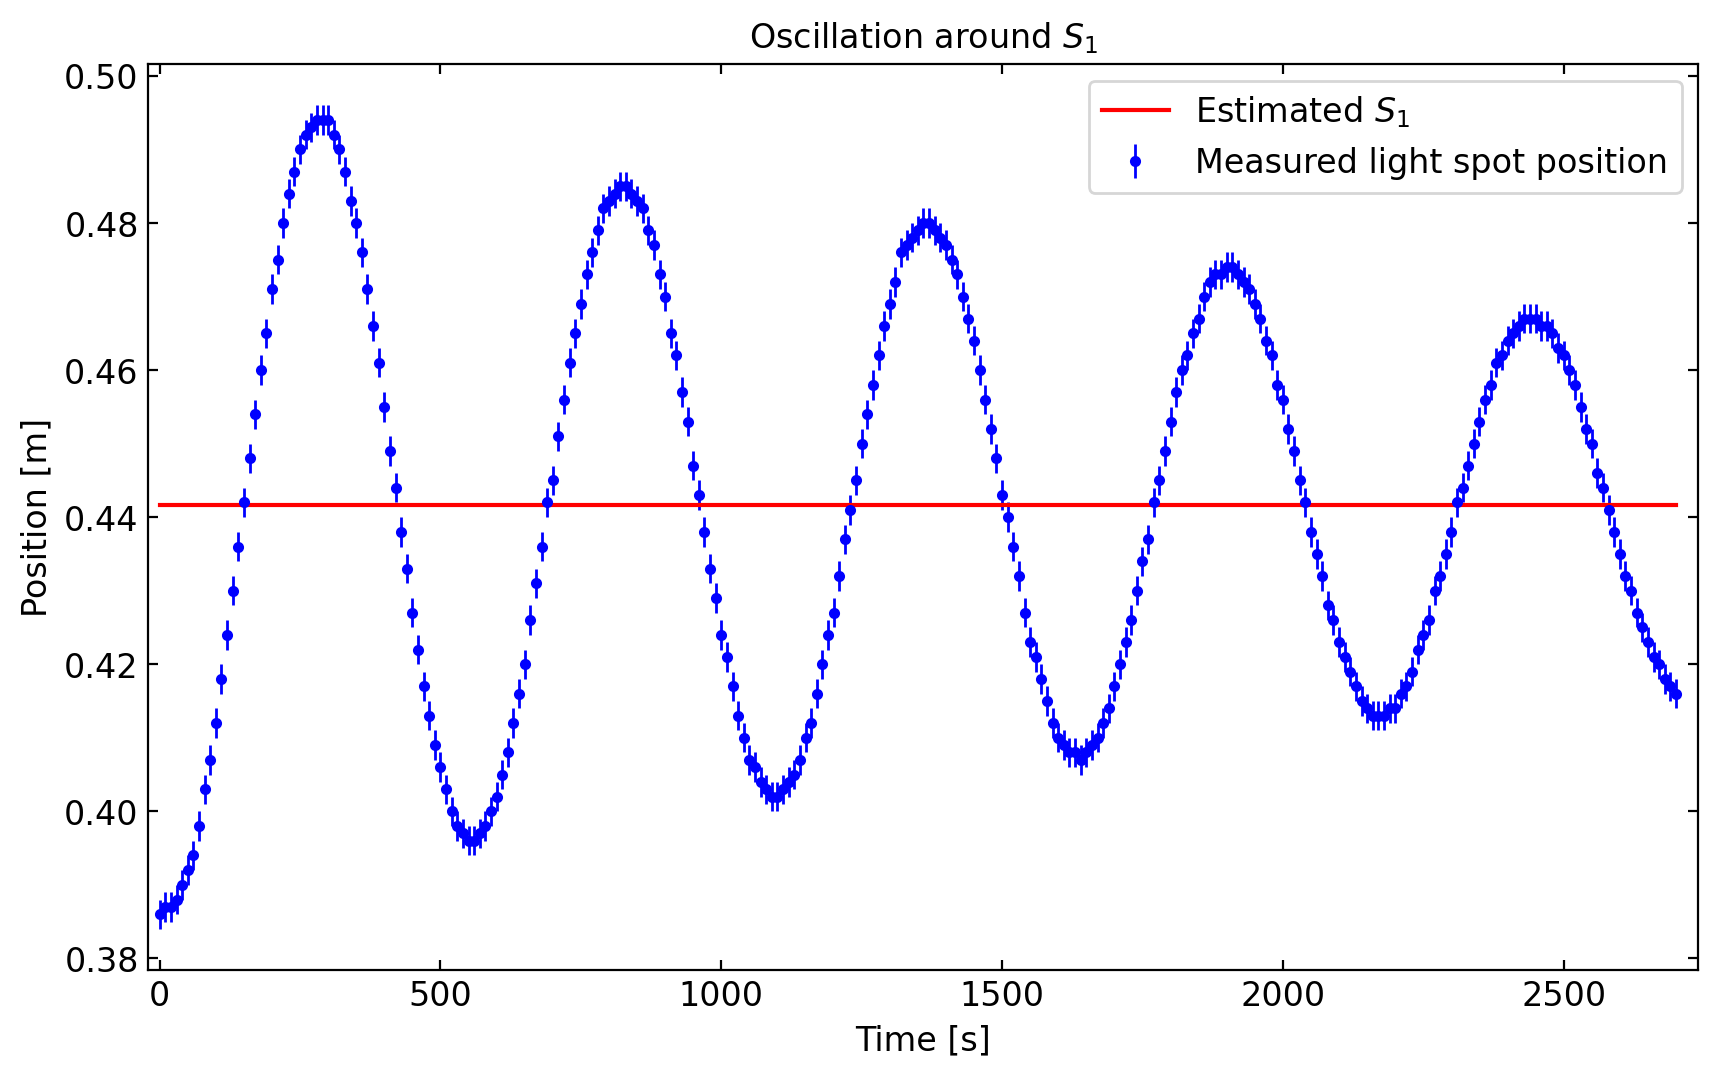
\includegraphics[width= 1 \linewidth]{figures/eq_s1.png}

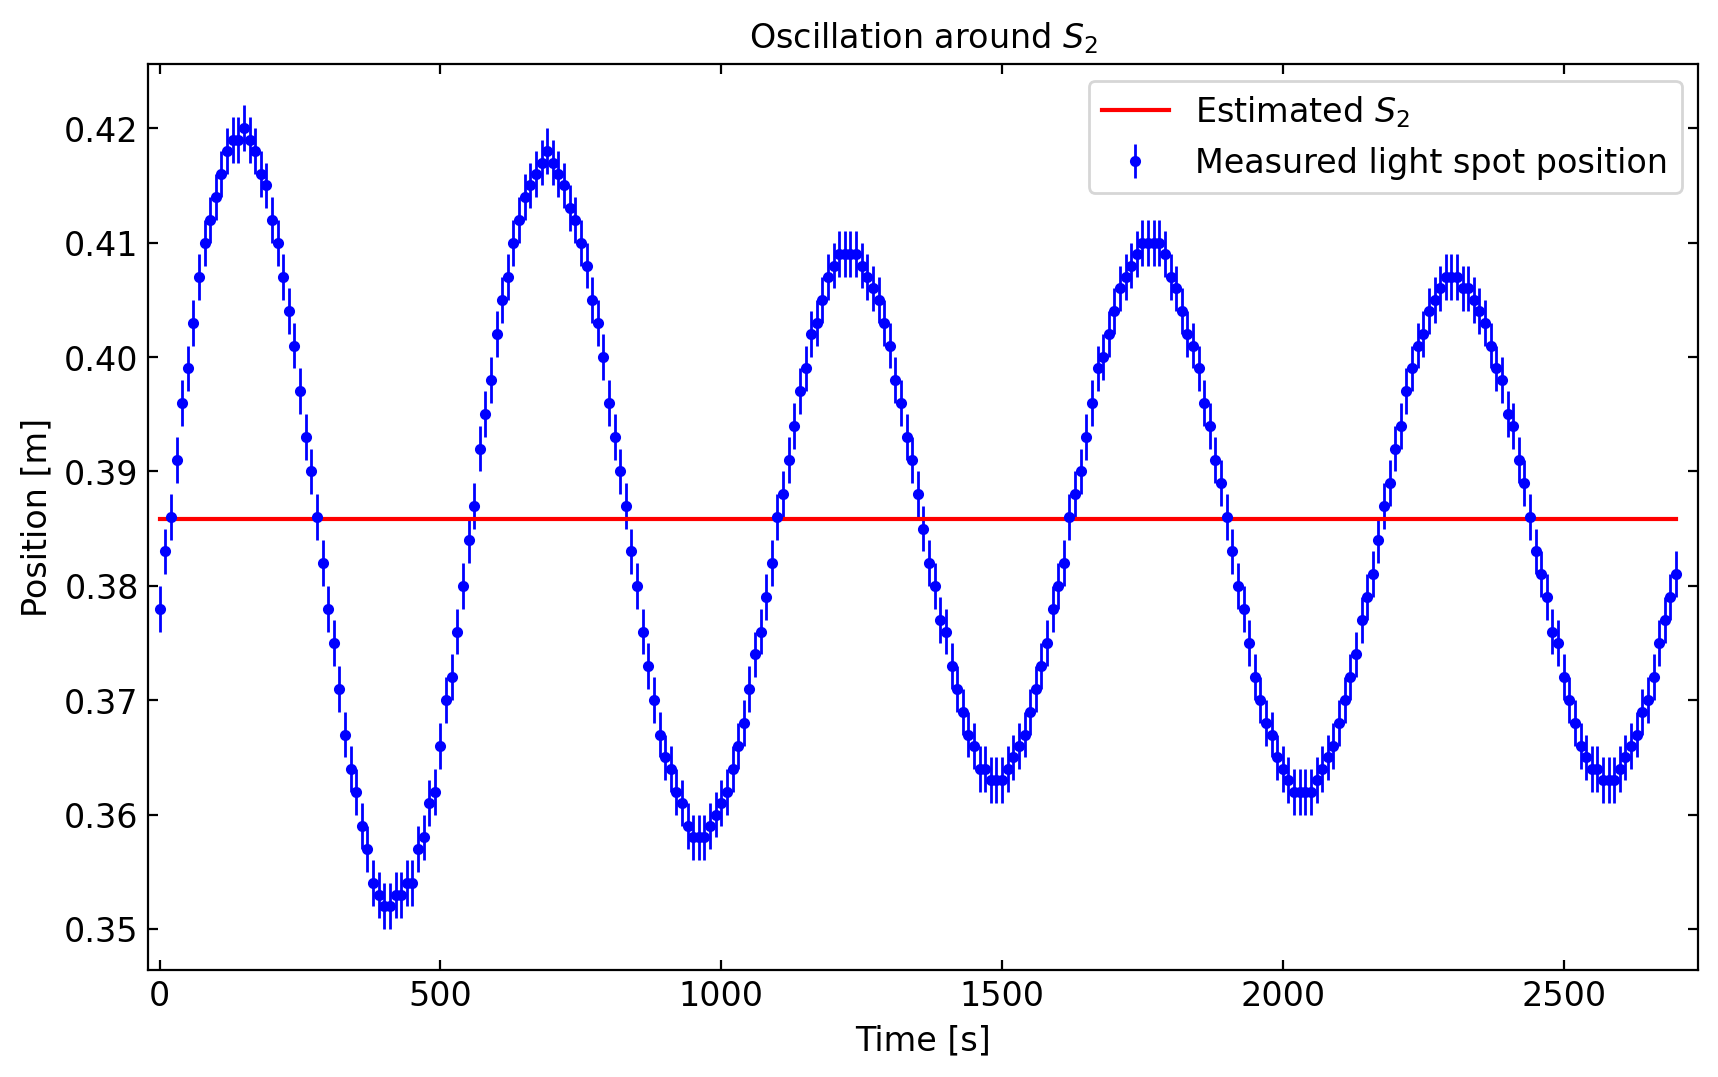
\includegraphics[width= 1 \linewidth]{figures/eq_s2.png}

Then we used first several data form $S_2$ measurement to determine the acceleration of the pendulum. 

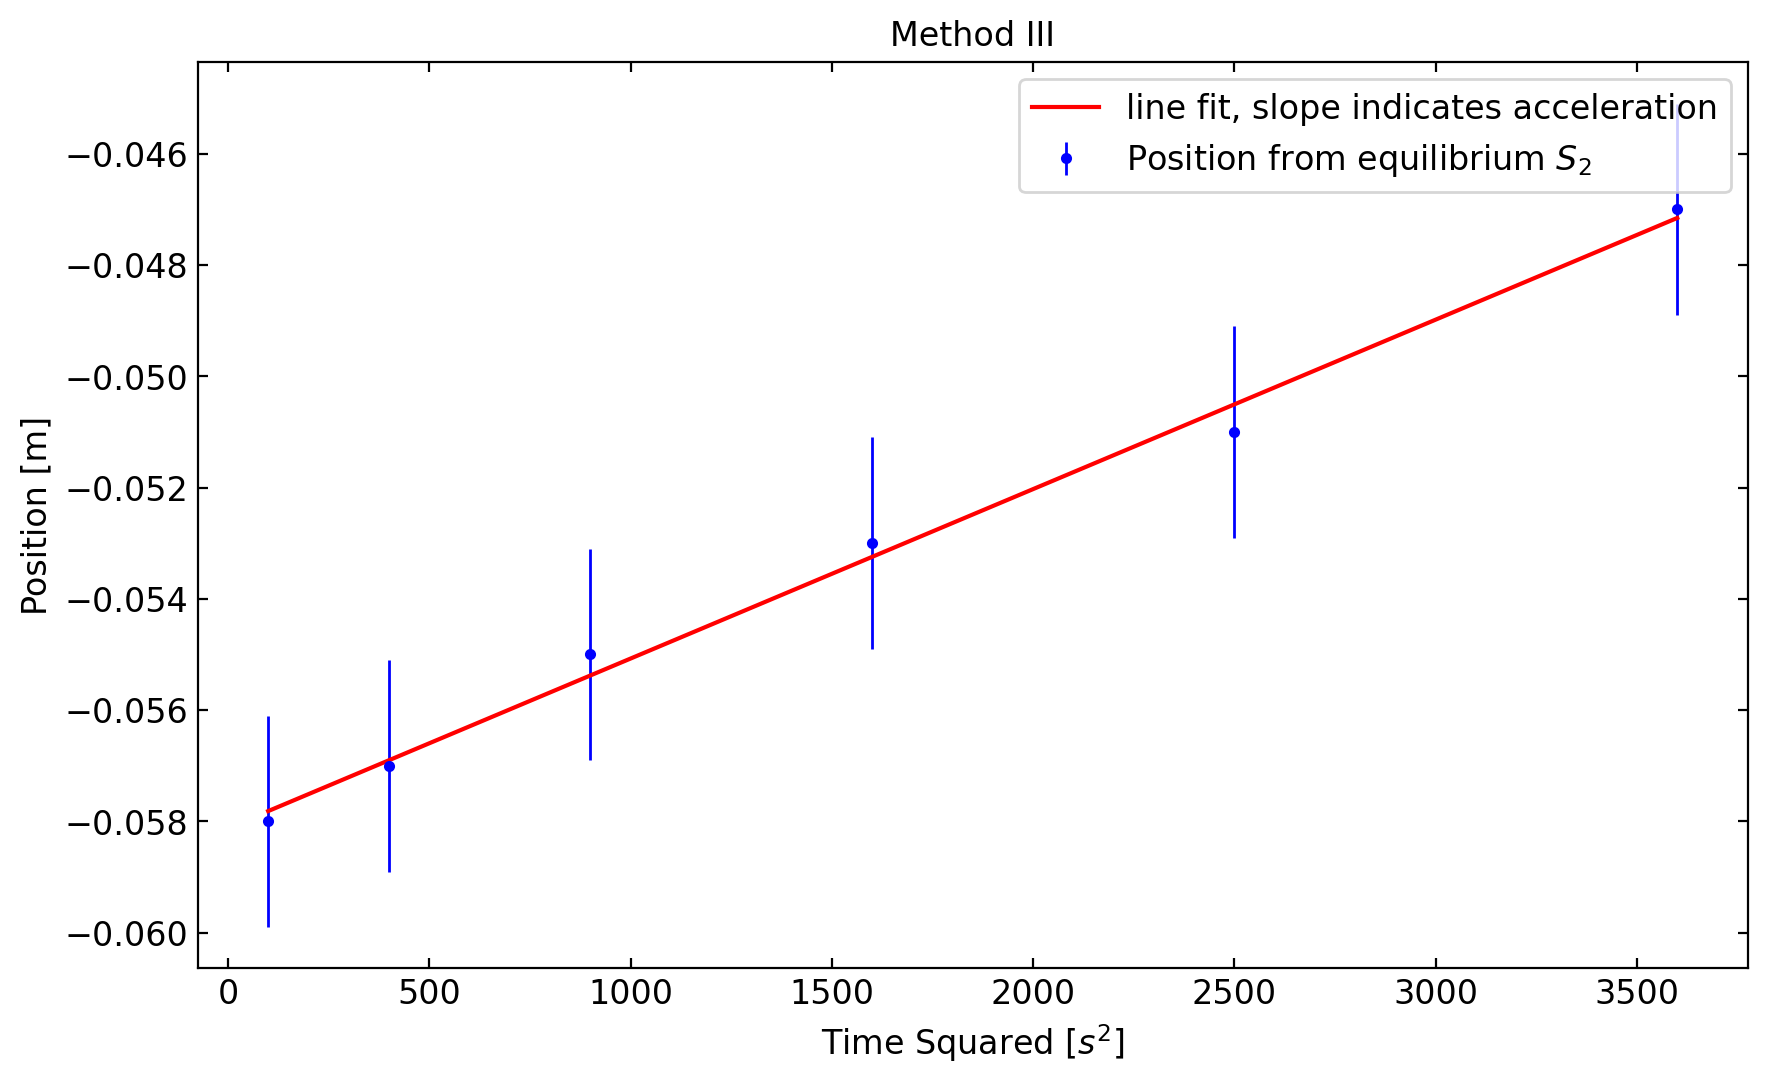
\includegraphics[width= 1 \linewidth]{figures/fit_m3.png}

Our data indicated that the measured $G = 4.13 \times 10^{-11}$ m$^3$ kg$^{-1}$ s$^{-2}$ values with the available PASCO equipment is within $34\%$ error to the accepted value $G = 6.674 \times 10^{-11} $ m$^3$ kg$^{-1}$ s$^{-2}$.

\newpage
\section{Theory and Setup}

\subsection{Set up and Procedure}
The Cavendish Torsion Balance experiment consisted of a torsion balance, which was a metal rod suspended from a wire, with two small spheres attached to the ends of the rod. The torsion balance was suspended inside a metal frame and positioned so that the two spheres were located close to two larger spheres of metal, which were placed on the sides of the frame. 

To measure the gravitational constant, we rotated the massive level-arm and carefully measured the amount of twist produced in the torsion balance. This was achieved by measuring the deflection of a small mirror attached to the rod. The deflection of the mirror was proportional to the amount of twist in the wire, which was caused by the gravitational force between the two spheres.

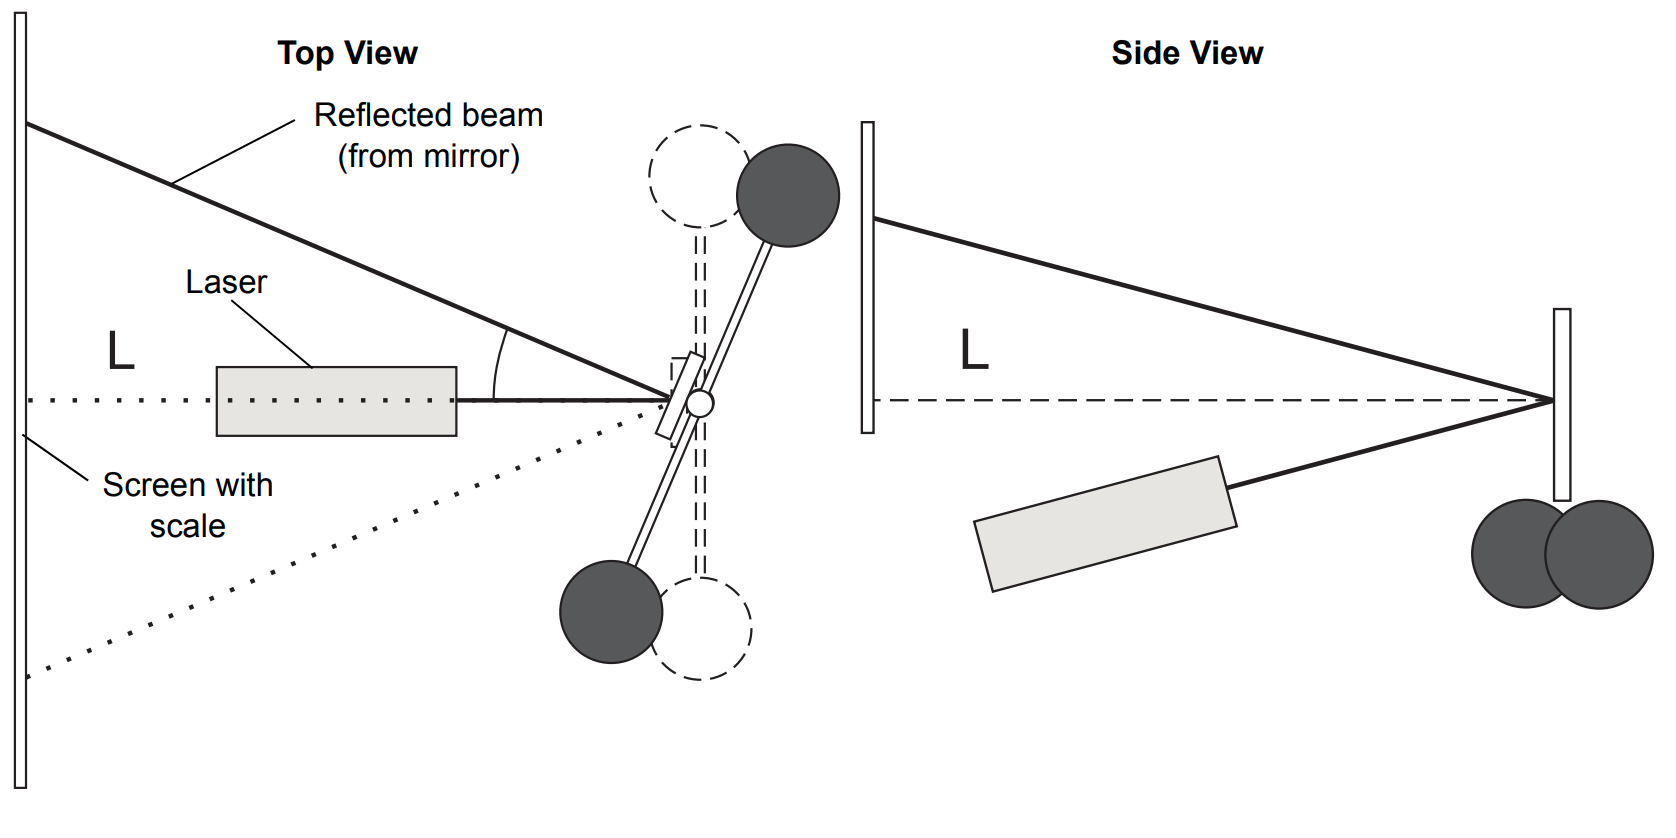
\includegraphics[width= 1 \linewidth]{figures/setup.png}

\subsection{Method 3}
We focused on method III in the lab manual to determine gravitational constant. 
In method III, we obtain the expression for G from eq. 3.4
$$G = \frac{b^2a_0}{2m_1}$$
where
$$a_0 = \frac{\Delta S d}{t^2 L}$$


\subsection{Error Propagation}
$$G = \frac{b^2 \Delta S d}{2 m_1 t^2 L}$$

\subsubsection{**Parameters**}

$\Delta S = ?$ (displacement between equilibrium positions $S_1$ and $S_2$)

$L = ?$ (distance between mirror and screen)

$t = ?$ (time difference for displacement under gravitational attraction)

$b =  42.2 $ mm (distance between the centers of the two masses)

$d = 50 $ mm (length of the lever arm of the pendulum bob crosspiece)

$r = 9.55 $ mm (radius of small balls, $8.19$ mm on page 3)

$m_1 = 1.5 (\pm 0.01)$ kg (mass of large mass)


\subsubsection{**Correction**}

Due to mutual interaction between the bigger spheres, we computed the correction to the torsion. The correction value, $\beta$, is

$$ \beta = \frac{b^3}{(b^2 + 4d^2)^{3/2}} $$

So we will get the corrected $G_0$ as

$$ G_0 = \frac{G}{1 - \beta } $$




\subsubsection{**Error**}
$$\sigma_G = \sqrt{\sum _i \left(\frac{\partial G}{\partial q_i}\sigma_{q_i}\right)^2}$$

$$\frac{\partial G}{\partial \Delta S} = \frac{b^2 d}{2 m_1 t^2 L}$$

$$\frac{\partial G}{\partial t} = -\frac{b^2 \Delta S d}{m_1 t^3 L}$$

$$\frac{\partial G}{\partial L} = -\frac{b^2 \Delta S d}{2 m_1 t^2 L^2}$$

$$\frac{\partial G}{\partial m_1} = -\frac{b^2 \Delta S d}{2 m_1^2 t^2 L}$$



$$\sigma_{\Delta S} = \sqrt{\left(\frac{\partial\Delta S}{\partial S_1}\sigma_{S_1}\right)^2+\left(\frac{\partial\Delta S}{\partial S_2}\sigma_{S_2}\right)^2}=\sqrt{2}\sigma_{S_1}=\sqrt{2}\sigma_{S_2}$$


\newpage
\section{Result and Analysis}
\subsection{Experiment Result}
We obtained data for relative position v.s. time squared. By method 3,
$$a_0\propto \frac{\Delta S}{t^2}$$

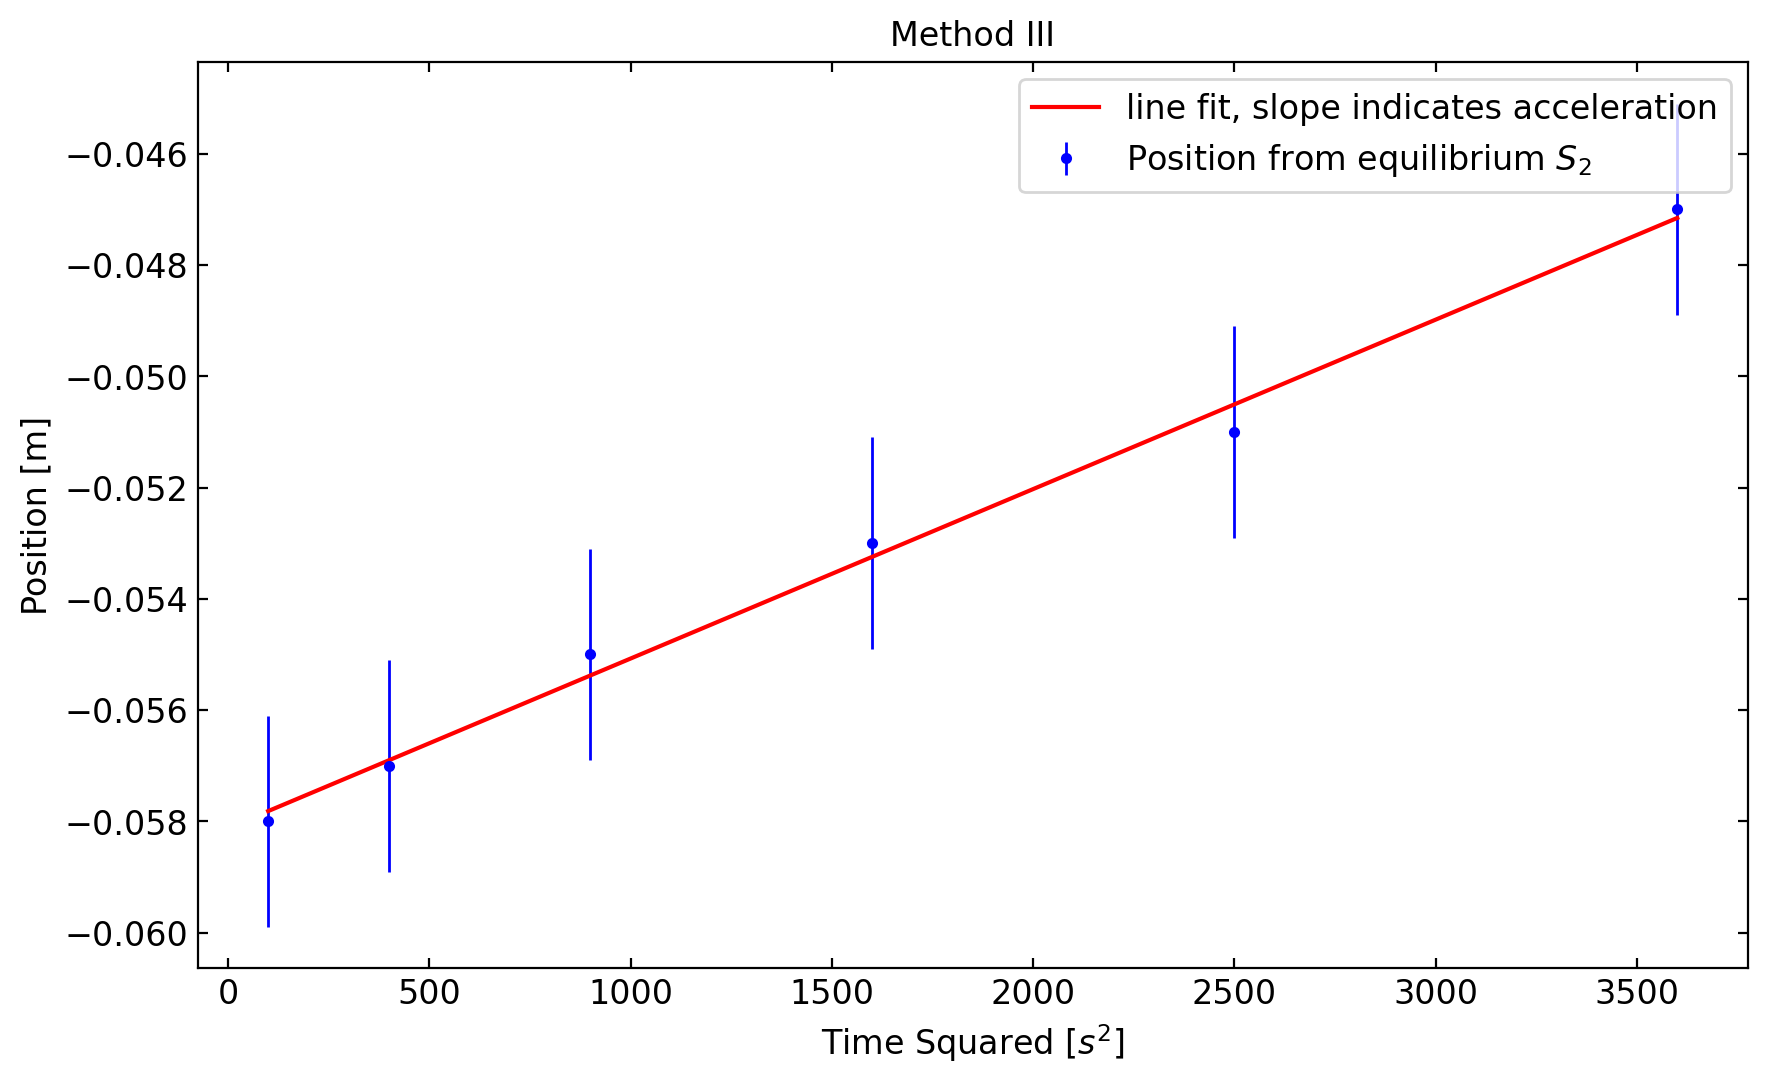
\includegraphics[width= 1 \linewidth]{figures/fit_m3.png}

\begin{center}
        \centering
        \begin{tabular}{|c |c |}
            \hline
        Time Stamp Squared $t^2$:  (s$^2$) & Distance $\Delta S$ from the Equilibrium Position (m) \\
\hline     \hline
            100 & -0.058\\
            \hline
            400 & -0.058\\
            \hline
            900 & -0.055\\
             \hline
            1600 & -0.053 \\
            \hline
            2500 & -0.051 \\
            \hline
            3600 &  -0.047\\
            \hline
        \end{tabular}
        \caption {Distance between neighboring extrema and their time span}
        \label{tab:my_label}
\end{center}
We determined the proportion constant by scipy.curve\_fit, and estimated gravitational constant to be $G_0 \approx 4.39 \times 10^{-11} \; \si{m^2.kg^{-1}.s^{-2}}$

Error
$$\delta a_0 = \sqrt{\left(\frac{d}{L}\delta \si{slope}\right)^2+\left(-\frac{\si{slope} \cdot d}{L^2}\delta L\right)^2}\approx 1.46\times 10^{-8} \;\si{m/s^2}$$
$$\delta G = \sqrt{\left(\pdv{G}{a_0} \right)^2 (\delta a_0)^2 + \left(\pdv{G}{m_1} \right)^2 (\delta m_1)^2 }\approx 8.67\times 10^{-12}\; \si{m^2.kg^{-1}.s^{-2}}$$
$$\delta G_0 = \frac{\G}{1-\beta} \approx 9.21\times 10^{-12} \; \si{m^2.kg^{-1}.s^{-2}}$$

\subsection{Error Analysis}
With our uncertainty, $G_0 = (4.39\pm 0.92)\times 10^{-11}\;\si{m^2.kg^{-1}.s^{-2}}$. Which deviates form the accepted value ($6.67\times 10^{-11}\;\si{m^2.kg^{-1}.s^{-2}}$) for about $30\%$. 

This cannot be explained by our statistical error. It is possible that we missed out on the initial few seconds of faster acceleration when we rotated the large masses, as we did not record the video immediately. However, this hypothesis may not hold true, as the acceleration during the first minute should be relatively constant.

Another potential error in our method is that we might have mistaken the very slow oscillation around 38.5 cm at the end of the $S_2$ calibration for equilibrium while waiting for it. When we rotated the position of the large masses during the slow oscillation, the small masses might not have been able to pick up enough acceleration due to the gravitational force pulling against the residual torque. This resulted in a smaller force and a corresponding smaller acceleration ($a_0$).

Electric potential fluctuation in the grounding wire might also contribute to it. Since the grounding wire of our device is connected with electronics in the room, which may result in a non-zero net charge in our device. So the rotation of balance will be repelled by the metal cage, and its acceleration decreases in general. Which may contributes to a lower estimation of gravitational constant. 


\newpage
\section{Discussion}

We conducted an experiment using the Cavendish torsion balance to determine the universal gravitational attraction constant, $G$. To do this, we measured the small masses' acceleration and deflection from equilibrium position by rotating the positions of the large masses. Our data indicated that the measured value of $G$ with the available PASCO equipment was $(4.39 \pm 0.86) \times 10^{-11}$ m$^3$ kg$^{-1}$ s$^{-2}$, which is significantly lower than the accepted value of $G = 6.674 \times 10^{-11}$ m$^3$ kg$^{-1}$ s$^{-2}$ by $34\%$. Our statistical error of $20\%$ cannot account for this deviation, so we propose that there may be potential systematic errors due to lagging in data recording and residual oscillation.

We identified potential sources of error as both statistical and systematic, including uncertainties in fitting acceleration data and calibration of the apparatus to equilibrium. We suggest improvements to the experiment, such as using more accurate methods like the final deflection and equilibrium position methods, with an error margin of $5\%$. We also propose using a more stable optical table to reduce susceptibility to external perturbations and improve the accuracy of equilibrium position readings.


%\hrulefill

%%%%%%%%%%%%%%%%%%%%%%%%%%%%%%%%%%%%%%%%%%%%%%%%%%%%%%%%

%\newpage
% \bibliographystyle{plain}
% \bibliography{lab_notes}

\end{document}